\section{Experiments}
\label{sec:experiments}


\paragraph{Dataset} We use KITTI dataset for our experiments.  \cite{geiger2013vision}. KITTI dataset is a labeled video sequence of road scenes under variety of driving conditions including highways and residential areas in Karlsruhe, Germany. It provides manually labelled ground truth data for localization of cars and also uses velodyne data provide metrically accurate estimates of cars location.


%%%%%%%%%%%%%%%%%%%%%%%%%%%%%%%%%%%%%%%%%%%%%%%%%%%%
\paragraph{Association error evaluation}

To verify the correctness of our association probability $\assocP$ we perform
association error experiment that compare the accuracy of point track
association with TPs with that of bounding box baseline method.

% \begin{align}
%   f^{i}_{reproj}&(\trackpj{t-1}, \lambda) =
%   \projectionOf{\invProjectionOf{\trackpj{t-1}}}\\
%   %&= K(R^i_t ((R^i_{t-1})^\top\lambda \ray - (R^i_{t-1})^\top T_{t-1}) + T_{t})\\
%   &= \frac
%   {p_{1:2}\lambda + q_{1:2}}
%   {p_{3}\lambda + q_{3}}
% \end{align}
% where $p_{1:3} = KR^i_t(R^i_{t-1})^\top\ray$ and
% $q_{1:3} = KR^i_t(R^i_{t-1})^\top T_{t-1} + KT_t$
% 
% Now that we have an association from TP $i$ to point track $j$ through
% $\lambda$, we can come up with an association probability
% \begin{align}
%    \assocP &= \frac{(\max \{ 0, \nabla \occf^\top
% \ray \})^2 }{P_{\text{reflection}}}\lambdadist\\
% &=(\max \{ 0, \nabla \occf^\top \ray \})^2
%   \prod_{0}^{\lambda} (1 - f_{occ}(\lambda \ray))^{d\lambda}
% \end{align}

Note that the fraction $\assocP$ although called association probability does
not capture the entire information that we have available for compute
association of points to tracks. This above fraction is the association
probability given the hypothesized parameters of TP model. 

To compute the association probability between TP $i$ and
point track $j$ we must use re-projection error as well. When the association
$i$ and $j$ is right and the point of reflection is at depth $\lambda$ the
re-projection error must be zero \eqref{eq:reprojerror}, otherwise the error
becomes a measure of distance from the true solution.
The error terms can be converted to probability domain by considering the error
term as negative log of probability

\begin{align}
  P^{(ij)}_{\text{assoc by reproj}}(\lambda) = \frac{1}{Z}\exp(-\Ereproj(\lambda))
\end{align}

Using both the evidence terms we can write probability of association as
\begin{align}
  P^{(ij)}_{\text{assoc}} = \frac{1}{Z'}\int_0^{\infty} \assocP \exp(-\Ereproj(\lambda))d\lambda
  \label{eq:prob-assoc}
\end{align}

Once we have the probability of association we can compute the best possible
assignment of TP for each point. The points having very small association
probability are assigned to the background,
\begin{align}
  i^*_{j} = \argmin_{i} \int_0^\infty \assocP \Ereproj(\lambda) d\lambda
\end{align}

We use bounding box based assignment of point tracks to TPs as the baseline.
For the regions where the bounding boxes overlap, we assign the points to the
TP that has smaller mean depth then the competing bounding box.

\begin{table}
  \centering
  \begin{tabular}{lrrr}
    \toprule
    Algorithm & Total & Unoccluded cars & Occluded cars \\
    \midrule
    bounding box only & 0.21 & \textbf{0.03}  & 0.36\\
    Using $P^{(ij)}_{\text{assoc}}$ & \textbf{0.21} & 0.08 & \textbf{0.32}\\
    Using $\assocP{}$ & 0.23 & 0.09 & 0.34 \\
    Using $P^{(ij)}_{\text{assoc by reproj}}$ & 0.23 & 0.08 & 0.34\\
    \bottomrule
  \end{tabular}
  \caption{Association Experiment results. The error is in terms of fraction of points wrongly associated with objects, hence lower is better.}
\end{table}


\paragraph{Localization Experiment}
Localization is the main goal of our project. We estimate the position, orientation and dimensions of the car with our framework and compute the error in birds eye view domain along the ground plane. We report error in three metrics translation error (t) in meters per car, yaw error (yaw) in radians per car and dimension error is again meters per car.

% %\subsection{Qualitative Results}
% \begin{figure}
%         \includegraphics[width=\columnwidth]{results/Visualization/City/2011_09_26_drive_0009/single_window_contPtTracks_size_bboxOcc_yawTstepWiseInference/0000000061.png}
% \end{figure}
% \begin{figure}
%   \includegraphics[width=\columnwidth]{results/Visualization/City/2011_09_26_drive_0009/single_window_lane_size_bboxOcc_yawTstepWiseInference/0000000061.png}
% \end{figure}
% \begin{figure}
%   \includegraphics[width=\columnwidth]{results/Visualization/City/2011_09_26_drive_0009/single_window_contPtTracks_size_bboxOcc_yawTstepWiseInference/0000000063.png}
% \end{figure}

%\subsection{Quantitative results}

\begin{table}
  \centering
  \begin{tabular}{lrrr}
    \toprule
    Energy & t & yaw & dim \\
    \midrule
    lane+contPtTracksNoOcc+size+bbox+posT   & 3.80 & 0.91 & 1.58 \\
    lane+contPtTracks+size+bboxOcc+posT+col & \textbf{3.78} & 0.91 & 1.58 \\
    lane+contPtTracks+size+bboxOcc+posT     & 3.81 & 0.92 & 1.59 \\
    lane+size+bboxOcc+posT+col              & 3.92 & 0.91 & 1.15 \\
    lane+size+bboxOcc+posT                  & 3.83 & 0.90 & 1.14 \\
    lane+size+bbox+posT                     & 3.83 & 0.90 & \textbf{1.14} \\
    initialization                          & 3.79 & \textbf{0.86} & 1.64 \\
    \bottomrule
  \end{tabular}
  \caption{Localization experiment results with different combination of energies. We report error in three metrics translation error (t) in meters per car, yaw error (yaw) in radians per car and dimension error is again meters per car.}
\end{table}

